\documentclass[conference]{IEEEtran}
\IEEEoverridecommandlockouts
\usepackage{cite}
\usepackage{amsmath}
\usepackage{amssymb}
\usepackage{amsfonts}
\usepackage{algorithmic}
\usepackage{enumerate}
\usepackage{graphicx}
\usepackage{textcomp}
\usepackage{xcolor}
\usepackage{graphicx}
%\usepackage{subfigure}
\usepackage{caption}
\usepackage{subfig}
\def\BibTeX{{\rm B\kern-.05em{\sc i\kern-.025em b}\kern-.08em
    T\kern-.1667em\lower.7ex\hbox{E}\kern-.125emX}}
\begin{document}
\title{Photovoltaic System Reconfiguration Strategy For Mismatch Condition\\
  {\footnotesize \textsuperscript{}}}

\author{\IEEEauthorblockN{Dafang Zhao, Michiko Inoue, Ooshita Fukuhito}
  \IEEEauthorblockA{\textit{Graduate School of Science and Technology, Nara Institute of Science and Technology (NAIST) \\8916-5 Takoyama-cho, Ikoma, Nara, 630-0192 Japan}}}
%% \IEEEauthorblock\{dafang-z.yu7, kounoe, f-ooshita\}@is.naist.jp}}
%% \{dafang-z.yu7, kounoe, f-ooshita\}@is.naist.jp

%% \author{\IEEEauthorblockN{1\textsuperscript{st} Dafang Zhao}
%% \IEEEauthorblockA{\textit{Graduate School of Science and Technology} \\
%% \textit{Nara Institute of Science and Technology}}
%% \and
%% \IEEEauthorblockN{2\textsuperscript{nd} Michiko Inoue}
%% \IEEEauthorblockA{\textit{Graduate School of Science and Technology} \\
%% \textit{Nara Institute of Science and Technology}}
%% \and
%% \IEEEauthorblockN{3\textsuperscript{rd} Ooshita Fukuhito}
%% \IEEEauthorblockA{\textit{Graduate School of Science and Technolog} \\
%% \textit{Nara Institute of Science and Technology}}}

\maketitle

\begin{abstract}
  Power generation efficiency of photovoltaic(PV) system is reduced significantly under partial shading or solar cell damage  conditions. This efficiency losses affected by turning on bypass diode of PV panels, which called mismatch losses. Reconfiguration technology to reconfigure electrical series or parallel connection among PV panels can maximize power generation. Recently, an efficient reconfiguration method of PV panel connection to optimize power generation is proposed. The method first list candidate configurations and applies precise power simulations to the candidates. However, some of candidates might not be realized by given PV panels and the paper does not show any systematic way to identify such a feasibility. In this paper, we propose a very fast algorithm to check the feasibility with high accuracy.
%This paper proposes a reconfiguration strategy that finds an optimal configuration among mismatched PV array in a less computational time. This algorithm is very light and suitable for embedded device. The results show that compare with existed reconfiguration method under non-uniform shadow scenario proposed algorithm computes an optimized configuration with less computational time and very high accuracy.
\end{abstract}

\begin{IEEEkeywords}
  Photovoltaic system, mismathed power loss, reconfiguration, dynamical reconfiguration.
\end{IEEEkeywords}

\section{Introduction} \label{intro}
As constant fossil energy generation is increasing the crisis of fossil fuel depletion and serious pollution problems for the environment, 
%As fossil energy is constantly depleted and increasing a serious pollution problem for the environment, 
research and utilization on a green and renewable energy have become necessary for sustainable society and environment.
%to support human existence and guarantee a sustainable human development.
%As the world of fossil energy constantly exhausted and the increasingly serious environmental pollution, the research and utilization of renewable and green energy have become necessary means of survival and development of human being. 
Photovoltaic (PV) energy has received a significant attention since it is unlimited and easy to be scaled up. Thanks to extensive technology and research on photovoltaic energy generation, large scale photovoltaic energy generation systems have been deployed into many practical applications. However, PV arrays are sensitive to shading and PV cell's fault or aging. This means that when 
%interconnection of 
PV cells or modules do not uniformly generate power
%have identical properties
 or experience different irradiance conditions from one another, the PV array is in mismatch condition and could not efficiently generate power. In addition, the photovoltaic arrays under mismatched conditions will accelerate the aging and heating of PV cells and cause a short circuit of photovoltaic cells to further damage the PV array. In order to maximize power generation and also avoid damaging PV cells, we propose an algorithm that can reconfigure photovoltaic arrays.
 
In this paper, we use non-uniform irradiance levels to represent mismatch condition and analyze the efficiency of a PV system.
% under different shaded working condition. 
% Photovoltaic arrays operating in non-uniform irradiance levels may present multiple local maximum power points (MPPs) \cite{b1}, which are generated by turning on bypass diodes. By changing electrical connection among the panels to prevent activate bypass diodes is a recent appealing solution\cite{b2}.
Photovoltaic arrays operating in mismatch conditions could not efficiently generate power, and reconfiguration of  panel connection has been widely investigated to solve this problem \cite{b2}.

Some of works proposed optimized or efficient algorithms to reconfigure the connection of PV cells \cite{b3}\cite{b4}. However, these works assume a full reconfiguration ability among PV cells. In general, a PV array is a connection of multiple PV panels, each PV panel has multiple PV modules, and each PV module consists of multiple PV cells. One typical PV panel has 3 PV modules with 24 PV cells. To realize reconfiguration in PV cell level, a new PV panel architecture is required.

Recently, as practical solutions, reconfiguration in PV panels have been investigated \cite{b5}\cite{b10}. One PV panel typically has two (plus and minus) terminals, and a PV array is configured by connecting PV panels in series and/or parallel. Such a configuration is also realized using a switch among PV panels, and reconfigurations in PV panel level can be regarded as  practical solutions. However, the reconfiguration in PV panel level is more difficult than that in PV cell level. PV modules in the same PV panel can be individually bypassed by bypass diodes when some mismatch condition occurs, and it causes multiple maximal power points (MPPs) for one PV panel.  

A PV panel level reconfiguration using genetic algorithm is proposed in\cite{b5}. Though this can generate a new configuration, 
computing cost is too significant and the algorithm cannot generate the best configuration precisely. A fast reconfiguration
strategy for minimizing power losses is presented in \cite{b10}.
In this strategy, candidates for PV array configurations are first listed by some fast estimation method, and, for each candidates, precise power simulations are applied. However, some candidate configurations might not be feasible, that is, it is impossible to realize a designated PV array configuration with given PV panels, and there is no description of a systematic way to identify the feasibility. 

In this paper,  we propose an algorithm to identify feasibility for a given configuration with less computational time and high
accuracy.
%The main difficulty facing the reconfiguration problem is that some or even all panels can be subjected to partial shading and there may be more than one MPP for each panel. Moreover, the panels, and not modules, reconfiguration strategy has to be realized so that modules providing the highest power could be grouped separately\cite{b3} \cite{b4}.
%
%This procedure enables to detect panel's operating conditions, in more than two-strings, receiving different irradiance levels. The reconfiguration algorithm will analyzes panels' working conditions and reorganizes panels into different strings by different irradiance levels. However, in sparse of mismatching conditions, distribution of panels among different irradiance levels are not significant. For that, by increasing number of strings in the PV array and using exhaustive search can be a solution\cite{b3}. Another approach to optimize photovoltaic arrays is using genetic algorithm\cite{b5}. However, computing cost is too significant, and this algorithm can't detect best configuration precisely. A simplest reconfiguration strategy for minimizing mismatch losses is presented in \cite{b10}. In this strategy, an algorithm gives candidates for PV array reconfiguration, for each candidates we have conduct power simulations. But some candidates are not feasible, which means there isn't any configuration for PV array can be realized. Since the power simulation is very time consuming, based on existed work we want to reduce number of candidates to accelerate overall reconfiguration algorithm. In this paper we propose an algorithm can give optimal configuration and check feasibility with less computational time and high accuracy.  

\section{Photovoltaic Array} \label{array}
In this paper, we use the following model of PV arrays, modules, strings and panels as showed in Fig. \ref{fig1}. A PV array is formed by several parallel connected (PV) strings, and a string is formed by several series-connected PV panels. A PV panel is formed by three PV modules.
% connected in series with bypass diodes. 
And each bypass diode is connected in parallel with a module.
\begin{figure}[htbp]
\centerline{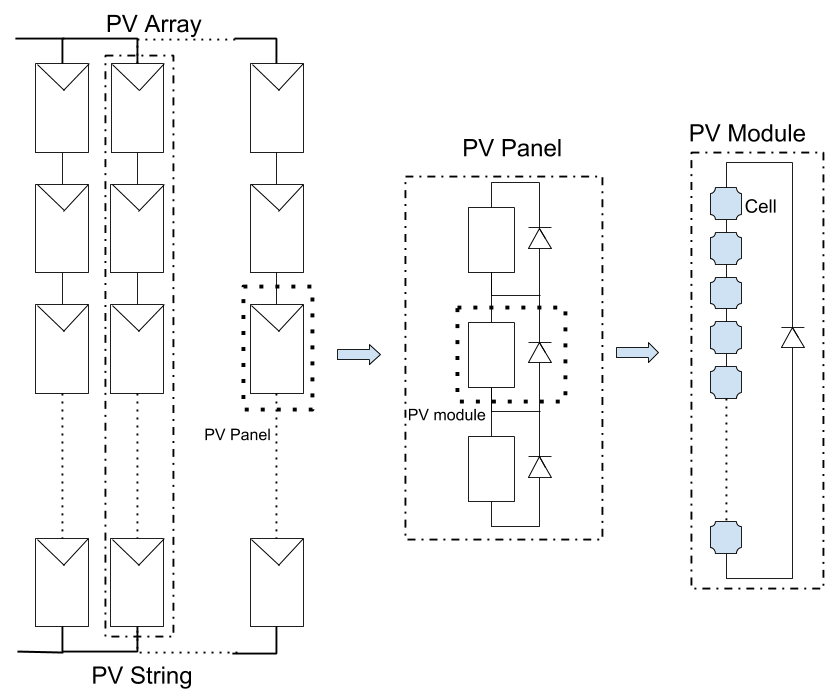
\includegraphics[width=7.2cm]{paper-fig1.png}}
\caption{PV arrays, strings, and panels.}
\label{fig1}
\end{figure}
\begin{figure}
\centering 
\subfloat[]{
	\label{fig2a}
	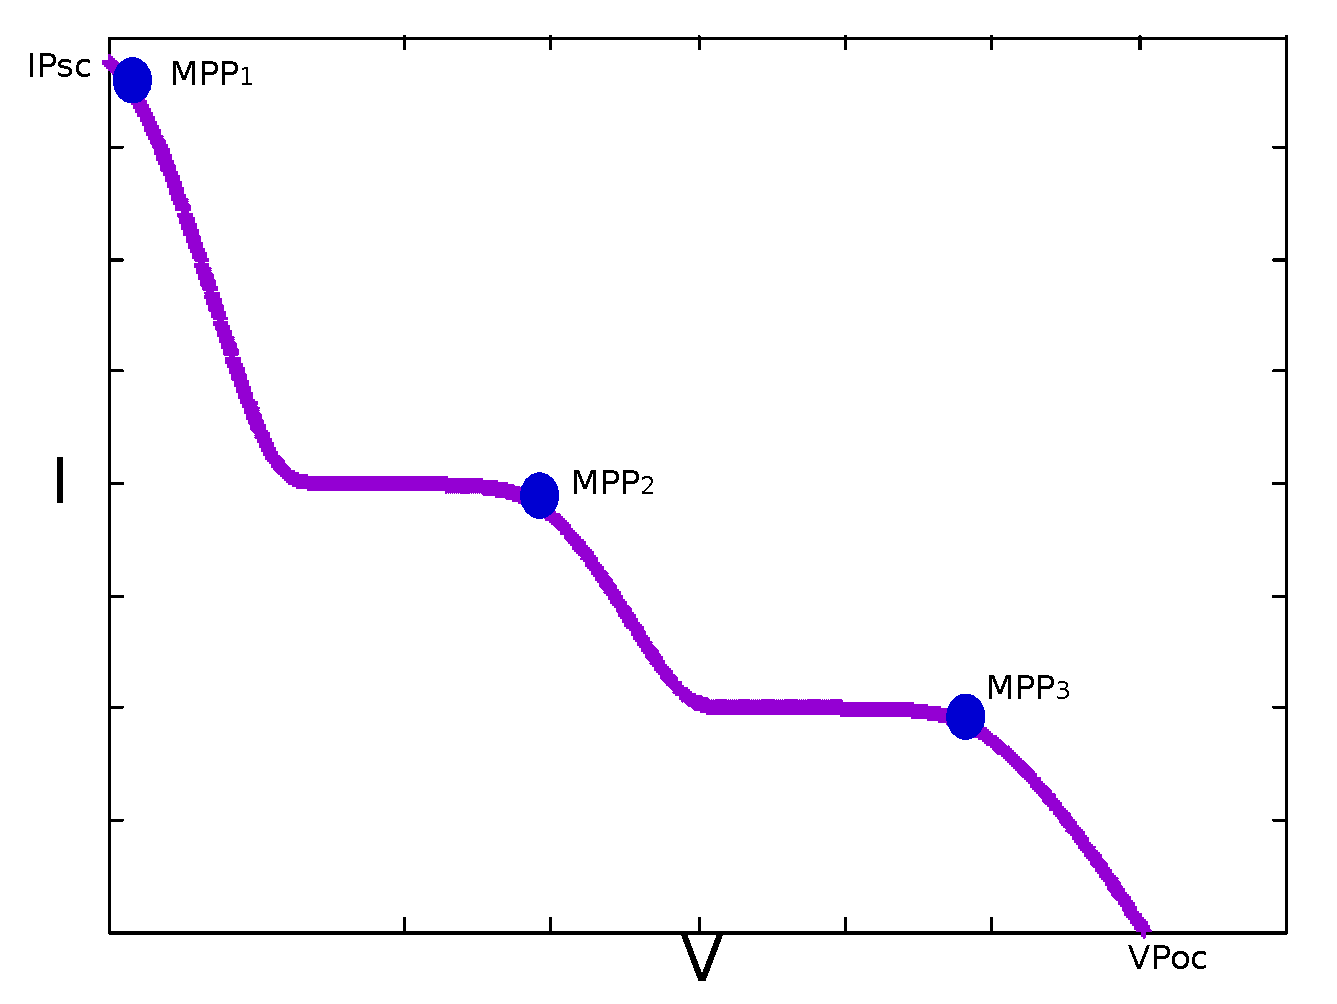
\includegraphics[width=4.2cm]{P2.pdf}
        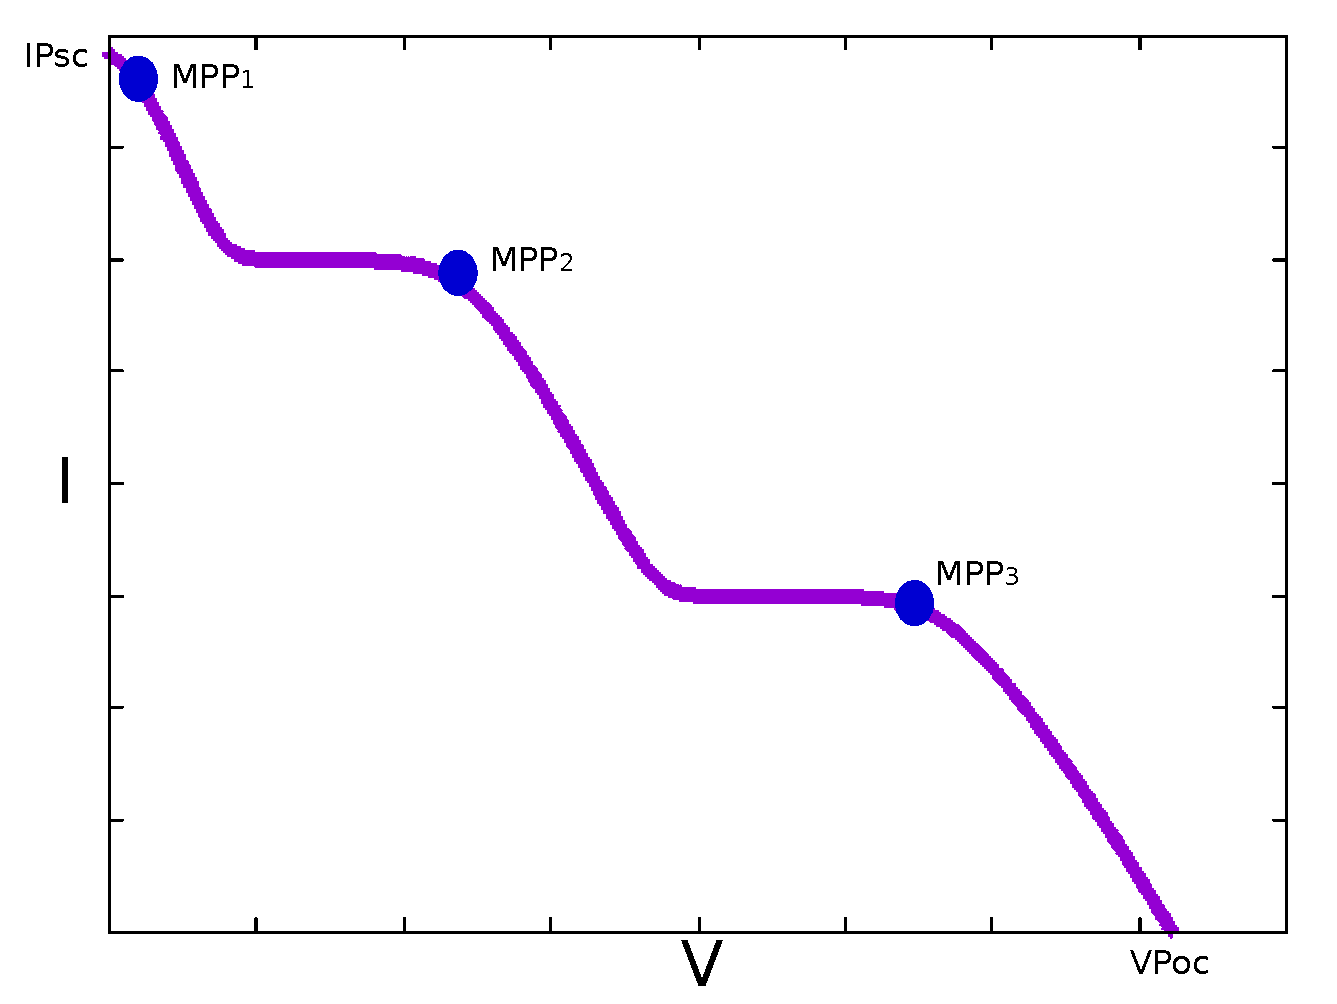
\includegraphics[width=4.2cm]{P1.pdf}}\\
\subfloat[]{
	\label{fig2b}
	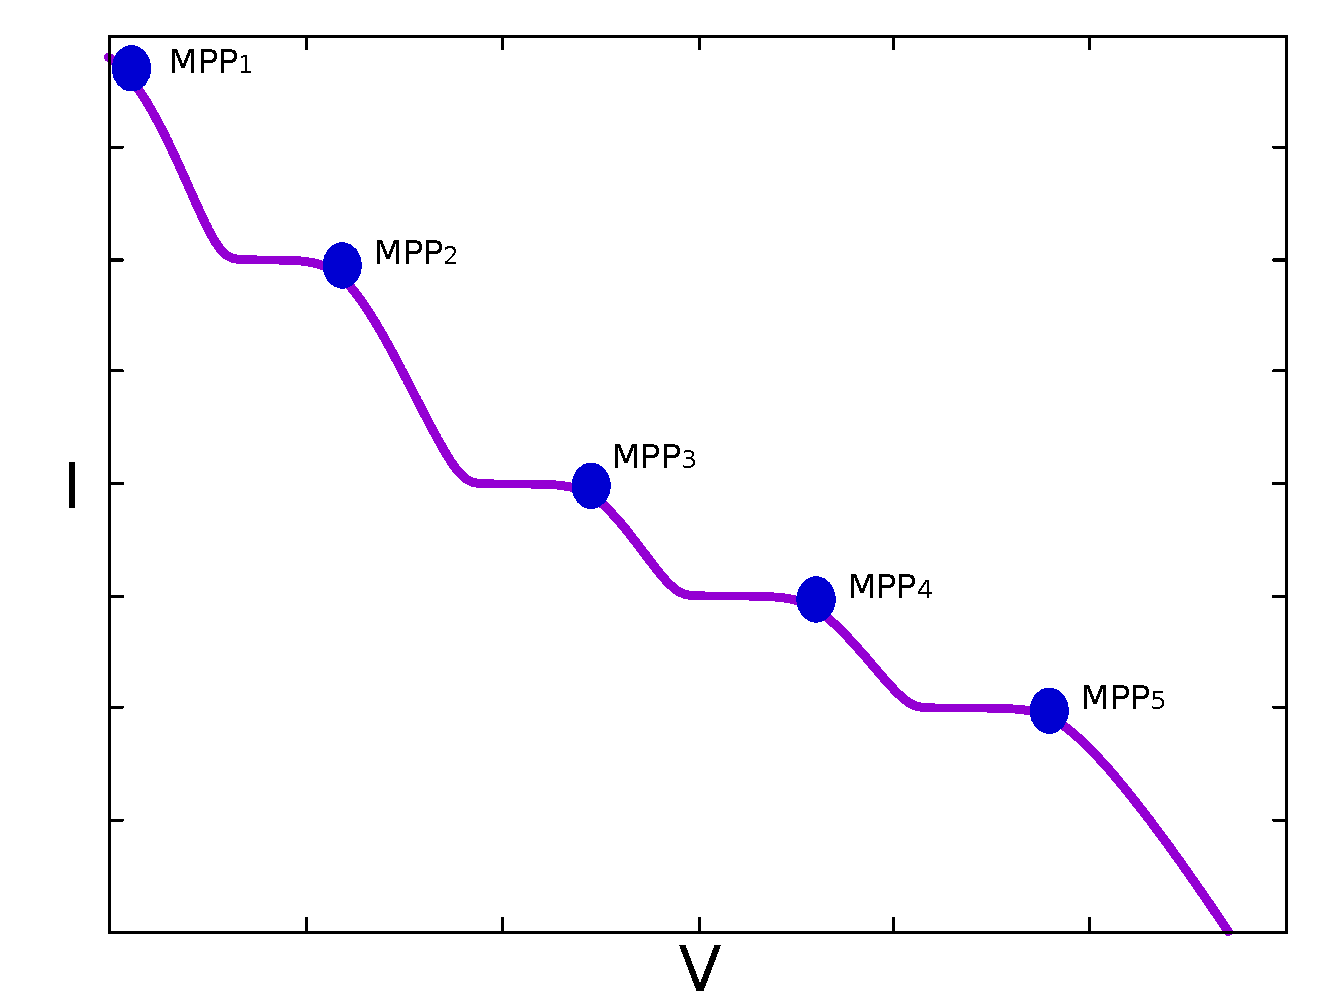
\includegraphics[width=4.2cm]{ser.pdf} }
\subfloat[]{
	\label{fig2c}
	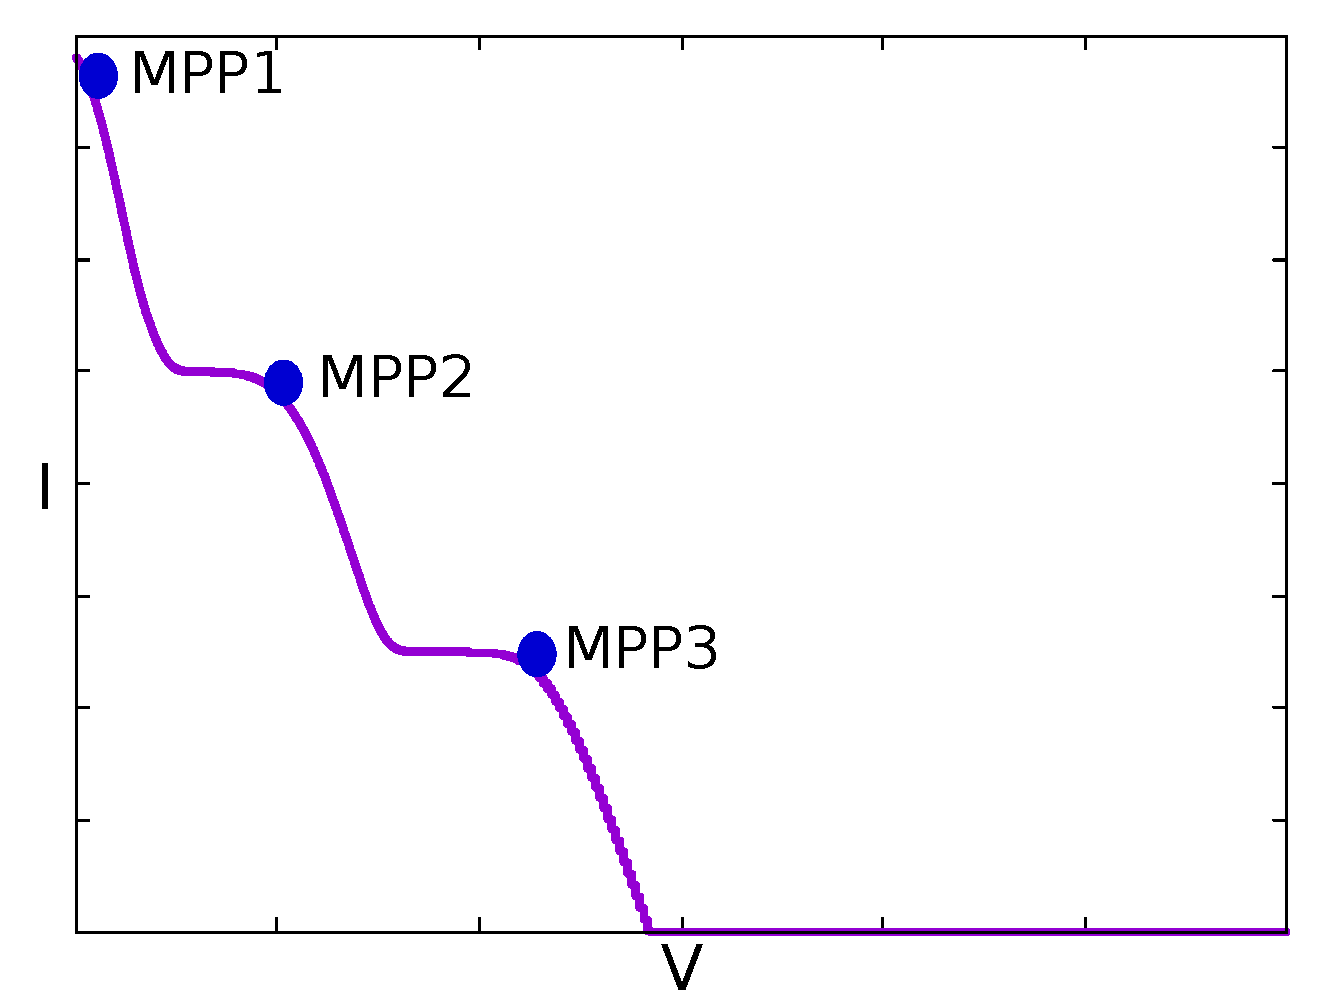
\includegraphics[width=4.2cm]{par.pdf}} \\
\caption{I-V curves, (a) 2 panels, (b) strings (series connection of PV panels), and (c) parallel connection of  PV panels}
\end{figure}
Fig.\ref{fig2a} shows  I-V curves for PV panels. PV panel generates a currents according to a provided control voltage within some range.
PV cells in a PV panel may have different conditions (irradiance or fault) and hence have different upper limits for their generated currents. Therefore, for lower control voltage, only PV cells that can generate higher currents can work and the other PV cells do not generate current with their bypass diodes switching on. As a result, PV panel might have multiple maximal power points (MPPs, points where power curve has extreme values). 
Fig.\ref{fig2b} and \ref{fig2c} show I-V curves for series and parallel connections of two PV panels. The series connection accepts wider range of control voltage, and the parallel connection can generate higher current. 
%When understanding complete I-V characteristics of some parallel and/or series connection of PV panels, we may need I-V characteristics of the PV panels. However, to find out the (near)  maximum generated power, it is enough to considers some restricted information including maximal power points (MPPs), a short circuit current, an open circuit voltage. These values form a fingerprint of the connection.

When understanding complete I-V characteristics of some parallel and/or series connection of PV panels, we may need I-V characteristics of the PV panels. However, to find out the (near) maximum generated power, it is enough to considers some restricted information including maximal power points (MPPs). The algorithm in \cite{b6} analyzes the current versus voltage (I-V) curves of panels and finds MPPs, short circuit current, open circuit voltage of each panel in mismatched conditions. These values form a fingerprint of the connection.

%We assume that each panel follows: The current versus voltage (\textit{I-V}) curve is acquired and calculated by algorithm presented in \cite{b6}. That algorithm will analyzes the panel \textit{I-V} curve sample by finding almost-constant-current and voltage regions and coordinate multiple maximum or minimum power point in the \textit{P-V} curve if PV array is working in mismatched conditions or not. 

%In mismatched conditions, the power versus voltage (P-V) curve of each panel shows multiple MPPs (maximal power points). We refer to a MPP by a pair $(V_{mpp},I_{mpp})$ where $V_{mpp}$ and $I_{mpp}$ are the voltage and the current that give a maximal power, respectively. The algorithm in \cite{b6} analyzes the current versus voltage (I-V) curves of panels and finds MPPs of each panel in mismatched conditions.


%All the panels in PV array have the same number (\textit{N}) of modules. For particular module, using (\textit{$V_{mpp_n}$, $I_{mpp_n}$}) to identify voltage and current values on different maximum power point by index \textit{n}. Those parameters can be directly estimated by the prosess provided in\cite{b7}.


%Furthermore, it is also assumed that for each string it has same number of panels. Means every string in PV array have same length. String's length are identical based on when they connected in parallel, a string has more panels may cause current back flow into other strings which have less panels\cite{b8}.
\section{Related Works}
Carotenuto et al. proposed a online recording method of PV module fingerprint \cite{b6}. In their method, a fingerprint including the current and voltage at open- and short-circuit points and multiple MPPs are obtained from several samples from a monitored PV panel. Orozco-Gutierrez et al. proposed a method to estimate multiple MPPs of a PV array from fingerprints of PV panels in the PV array \cite{b7}.

Orozco-Gutierrez et al. further proposed a Fast reconfiguration algorithm to optimize power generation by reconfiguring the connection of PV panels \cite{b10}, where the online monitoring \cite{b6} and the power estimation \cite{b7} are utilized. In the method in \cite{b10}, first, close values of fingerprints from monitoring of PV panels are grouped with some representative values, and then possible combinations of reconfiguration are enumerated. Their power values are estimated by \cite{b7} along with careful estimation of possible errors. The method presented a simple feasibility check and obtains estimated power values for all the possible connections for representative values with some error rate \textit{err}, and then select configurations within \textit{err} difference from the largest estimated value as candidates of the optical configurations. 
\begin{table}[htbp]
\caption{DATASET OF PARTIAL-SHADING PV ARRAY}
\begin{center}
\begin{tabular}{cccc}
%\multicolumn{4}{c}{DATASET OF PARTIAL-SHADING PV ARRAY} \\ \hline \hline
Panels & Vmpp(V)                & Impp (A)            & MPP(W)                 \\ \hline
P1     & {[}0, 2.9, 11.4{]}     & {[}0, 0.5, 2{]}     & {[}None, 1.5, 22.8{]}     \\
P2     & {[}2.9, 17.1, 17.1{]}  & {[}0.5, 3, 3{]}     & {[}1.5, 51.3, 51.3{]}  \\
P3     & {[}2.9, 2.9, 2.9{]}    & {[}0.5, 0.5, 0.5{]} & {[}1.5, 1.5, 1.5{]}    \\
P4     & {[}0, 11.4, 11.4{]}    & {[}0, 2, 2{]}       & {[}None, 22.8, 22.8{]}    \\
P5     & {[}0, 2.9, 11.4{]}     & {[}0, 0.5, 2{]}     & {[}None, 1.5, 22.8{]}     \\
P6     & {[}2.9, 11.4, 11.4{]}  & {[}0.5, 2, 2{]}     & {[}1.5, 22.8, 22.8{]}  \\
P7     & {[}2.9, 11.4, 17.1{]}  & {[}0.5, 2, 3{]}     & {[}1.5, 22.8, 51.3{]}  \\
P8     & {[}11.4, 11.4, 11.4{]} & {[}2, 2, 2{]}       & {[}22.8, 22.8, 22.8{]} \\
P9     & {[}2.9, 11.4, 17.1{]}  & {[}0.5, 2, 3{]}     & {[}1.5, 22.8, 51.3{]} 
\end{tabular}
\label{tab1}
\end{center}
\end{table}

\section{Reconfiguration Algorithm} \label{algo}

\subsection{Overview of the algorithm}
In this section, we describe the overview of the Fast reconfiguration algorithm in \cite{b10}. First, the reconfiguration algorithm determines MPPs for PV modules in the mismatched condition by using algorithms in \cite{b6}\cite{b7}. As an example, we consider a PV array where nine panels are connected in three strings. We assume that, in this example, the reconfiguration algorithm finds MPPs given in Table \ref{tab1}.
%To reconfigure a large scale partial shading PV array, an example refers to 9 panels which have been connected in 3 strings. In this example, mismatching conditions presented in Table \ref{tab1}. 
%Each panel made of 3 identical PV modules (\textit{N=3}), dataset in Table \ref{tab1} are provide by method in \cite{b6} \cite{b7}. As described in \cite{b10}, the Fast reconfiguration strategy firstly determine \textit{$V_{mpp}$} and \textit{$I_{mpp}$} for each PV module by using the algorithm in \cite{b7} \cite{b9}. 
After that, the Fast reconfiguration algorithm generates candidates of current assignments 
%% where the current assignment specifies a current of each string. The reconfiguration algorithm
and treats the current of each MPP as a current candidate for string, constructs a current assignment by assigning a current candidate to each string. The reconfiguration algorithm generates current assignments by considering all combinations of current candidates for string.
%Then determine MPP current and voltage candidates among PV array. Calculate MPP candidates matrix by multiplying the current and voltage candidates. 
Then, for each current assignment, the reconfiguration algorithm computes the number of working modules (\textit{$Q_{M_n}$}) in each string. We define a configuration as a combination of a current assignment and the number of working modules in each string. MPP candidates are presented in (\ref{mpp}) and number of working modules for each string are presented in (\ref{qmn}), respectively. 

\begin{equation}
\begin{aligned}
\textit{MPP candidates}& = \\ [\{ 0.5, &0.5, 2\}, \{0.5, 2, 2\}, \{2, 2, 2\}, \{2, 2, 3\}]
\end{aligned}\label{mpp}
\end{equation}
\begin{equation}
\begin{aligned}
\textit{$Q_{M_n}$} = &  [\{8, 8, 8\}, \{7, 7, 7\}, \{5, 5, 5\}, \{4, 4, 4\}]
\end{aligned}
\label{qmn}
\end{equation}
By this algorithm, we obtain a set of candidate configurations. Since we can estimate the generated power of each candidate configuration, we can select the candidate configuration that maximizes the generated power.
%\vspace{10cm}
%Using the number of working modules (\textit{$Q_{M_n}$}) for each MPP current candidates to determine MPP candidates. Finally the Fast reconfiguration strategy gives MPP candidates for reconfiguration, which specifies a current value and minimum number of working modules for each string in PV array. 
The general steps of Fast reconfiguration strategy as showed in Fig. \ref{flowchart}. 
\begin{figure}[htbp]
\centerline{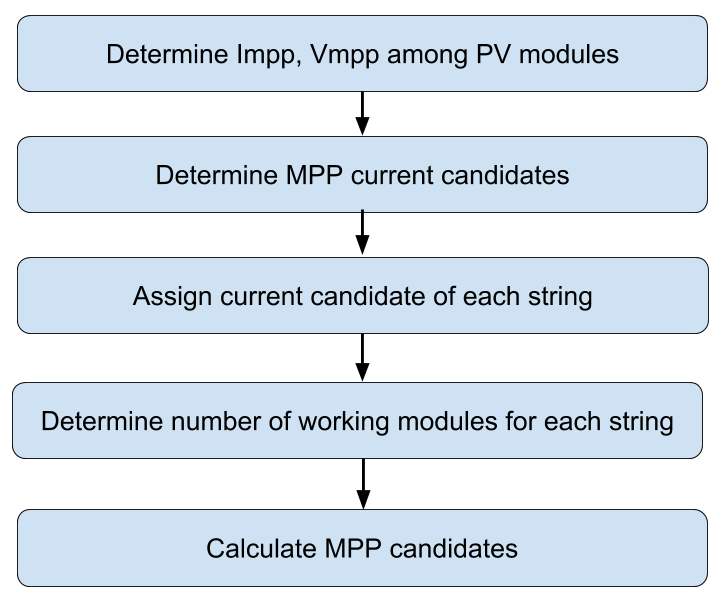
\includegraphics[width=8cm]{flowchart(1).png}}
\caption{Flowchart of reconfiguration algorithm in \cite{b10}.}
\label{flowchart}
\end{figure}
The previous estimation can not give precise reconfiguration answer. This algorithm lists some candidate configurations ( in addition to the maximum one ) and for each candidate configuration it will executes a time consuming and precise power simulation. Considering there are some errors in previous estimation, this algorithm is not efficient for finding the best configuration. 



\subsection{Feasibility Problem}\label{feasPro}
To execute a power simulation, we have to assign panels to each string to realize a candidate configuration. However, the way is not given in \cite{b10} and some candidate configurations are infeasible. 
The definition of feasibility in (\ref{feas}). When a configuration needs working modules in a string (\textit{$M_S$}) are less than number of working module per-string (\textit{$Q_{M_{n}}$}), then this configuration is infeasible. 
\begin{equation}
\left\{\begin{matrix}
M_S < Q_{M_{n}} & & \text{Infeasible}\\ 
M_S \geqslant Q_{M_{n}} & & \text{Feasible} 
\label{feas}
\end{matrix}\right. 
\end{equation}
For an configuration example \{0.5A, 0.5A, 2A\}, there are 8 PV modules working on each string. According to Table I, for a string current on 2A at least need 4 panels, remaining panels can not provide enough PV module working on 0.5A for another two strings. 
Of course we can compute it by using an exhaustive search. However, it is time-consuming. So, we need an algorithm to efficiently identify feasibility of a configuration and realize the configuration if it is feasible.

%Due to a PV panel can not be used into different string, those MPP candidates may have some un-feasible configurations. Our proposed algorithm based on the method in \cite{b10} to calculate MPP candidates and using unique panel selection technology to give optimal reconfiguration solution among partial-shading PV array. 

%In this example, though the procedure in Fast reconfiguration strategy, MPP candidates are presented in (\ref{mpp}) and number of working modules in MPP candidates are presented in (\ref{qmn}), respectively. 


%\begin{equation}
%\begin{aligned}
%\textit{MPP candidates} = [\{ 0.5, 0.5, 2\}, \{0.5, 2, 2\}, \{2, 2, 2\}, \{2, 2, 3\}]
%\end{aligned}\label{mpp}
%\end{equation}
%\begin{equation}
%\begin{aligned}
%\textit{$Q_{M_n}$} = &  [\{8, 8, 8\}, \{7, 7, 7\}, \{5, 5, 5\}, \{4, 4, 4\}]
%\end{aligned}
%\label{qmn}
%\end{equation}
\section{An Algorithm to Identify Feasibility}
In this section, we propose an algorithm to identify feasibility.
\subsection{The Input And Output Of Algorithm}
%First, we summarize the input and output of our algorithm. 
The input of our algorithm is information of a PV array and a configuration. The information of a PV array is given as a set of panels and the number of working modules in each panel for each current candidate. Table \ref{mpp3-1} shows the information of a PV panel given in Table \ref{tab1}. For example, this table shows panel P2 includes three, two, and two modules that work in current 0.5A, 2A and 3A, respectively. Recall that a configuration is a combination of a current assignment and the number of working modules in each string, and a current assignment specifies a current for each string. The output of our algorithm is feasibility of the given configuration. That is, the algorithm determines whether there exists assignment of panels to strings that realizes the configuration.
\begin{table}[htbp] 
\caption{Information of a PV array}
\begin{center}
%\begin{equation}
%\begin{center}
\begin{tabular}{l|lllllllll}
    & P1 & P2 & P3 & P4 & P5 & P6 & P7 & P8 & P9 \\ \hline
0.5A & 2  & 3  & 3  & 2  & 2  & 3  & 3  & 3  & 3  \\
 2A & 1  & 2  & 0  & 2  & 1  & 2  & 2  & 3  & 2  \\
 3A & 0  & 2  & 0  & 0  & 0  & 0  & 1  & 0  & 1 
\end{tabular}\label{mpp3-1}
%\end{center}
%\end{equation}
\end{center}
\end{table}  
%\subsection{Feasibility}
%The feasibility of configuration based on the assumption of section \ref{array}, each string in PV array must have same number of panels. 
%Definition of feasibility in (\ref{feas}). When a configuration needs panels in a string (\textit{$NP_n$}) are over maximum number of panels per-string(\textit{$NP_{stMAX}$}) this configuration is unfeasible. 
%\begin{equation}
%\left\{\begin{matrix}
%NP_n > NP_{stMAX}& & \text{Unfeasible}\\ 
%NP_n \leq NP_{stMAX} & & \text{Feasible} 
%\label{feas}
%\end{matrix}\right. 
%\end{equation}
%For the first MPP candidate \{0.5, 0.5, 2\} need 8 modules for each string. According to Table \ref{tab1}, for a string current on 2A at least need 4 panels and didn't meet feasible requirement, thus, algorithm terminate. The second MPP candidate \{0.5, 2, 2\} as same as previous one also not feasible.
%Recall that a configuration is a combination of a current assignment and the number of working modules in each string, and a current assignment specifies a current for each string. The output of our algorithm is feasibility of the given configuration. That is, the algorithm determines whether there exists assignment of panels to strings that realizes the configuration.
\subsection{Panel Selection Strategy} \label{selection strategy}
Let $s$ be the number of strings, and $i_h$ ($0\le h<s$) be the current assigned to the $h$-th string. Without loss of generality, we assume $i_0\le i_1\le \cdots \le i_{s-1}$ holds. In our algorithm, we first determine the assignment of panels for the $(s-1)$-th string (i.e., the string with the highest current), and then determine assignments for $(s-2)$-th string, $(s-3)$-th string, and so on.

We explain the way to determine the assignment of the $(s-1)$-th string. To do this, we consider the number of working modules of each panel for currents less than $i_{s-1}$. Let $m_p(i)$ be the number of working modules of Panel $p$ that work in current $i$. For each panel $p$, we consider the difference vector $D_p=(m_p(i_{s-2})-m_p(i_{s-1}), m_p(i_{s-3})-m_p(i_{s-2}), \ldots, m_p(i_0)-m_p(1))$. The first element $d_1$ of $D_p$ means, if we use panel $p$ in current $i_{s-1}$, we lose $d_1$ working modules in current $i_{s-2}$. Then we sort panels in lexicographic order by vector $D_p$. This means, a panel with minimum module losses should firstly assign to the string with the highest current.
%... Sorry, I didn't complete this comment.
%\vspace{1cm}
%Calculate MPP candidates based on existed reconfiguration method in \cite{b10}. MPP current candidates and MPP voltage candidates are present in (\ref{e1}) and (\ref{e2}), respectively. Additional, number of real working module at MPP current candidates are given in (\ref{e3}). Due to 5\% error of MPP current candidates and 18\% error of MPP voltage candidates, total error rate of MPP candidates is 23\%. Though procedure of algorithm in \cite{b10}, MPP candidates with 23\% are: [\{ 0.5, 0.5, 2\}, \{0.5, 2, 2\}, \{2, 2, 2\}, \{2, 2, 3\}] and require working modules per strings are: [\{8, 8, 8\}, \{7, 7, 7\}, \{5, 5, 5\}, \{4, 4, 4\}].
%\begin{equation}
%\begin{aligned}
%\textit{$I_{mpp_n}$} = [&\{  \text{$0.5_{(9)}$}, \text{$0.5_{(9)}$}, \text{$0.5_{(9)}$}   \}, \{ \text{$0.5_{(9)}$}, \text{$0.5_{(9)}$}, \text{$2_{(11)}$} \},  \\ &\{\text{$0.5_{(9)}$}, \text{$0.5_{(9)}$}, \text{$3_{(4)}$} \}, \{\text{$0.5_{(9)}$}, \text{$2_{(11)}$}, \text{$2_{(11)}$} \}, \\ & \{\text{$0.5_{(9)}$}, \text{$2_{(11)}$}, \text{$3_{(4)}$} \}, \{\text{$0.5_{(9)}$}, \text{$3_{(4)}$}, \text{$3_{(4)}$} \}, \\ &\{\text{$2_{(11)}$}, \text{$2_{(11)}$}, \text{$2_{(11)}$} \}, \{\text{$2_{(11)}$}, \text{$2_{(11)}$}, \text{$3_{(4)}$} \}, \\ & \{\text{$2_{(11)}$}, \text{$3_{(4)}$}, \text{$3_{(4)}$} \}, \{\text{$3_{(4)}$}, \text{$3_{(4)}$}, \text{$3_{(4)}$} \}] \pm 5\%  \label{e1}
%\end{aligned}
%\end{equation}
%\begin{equation}
%\begin{aligned}
%\textit{$V_{mpp_n}$} = [&12.4, 24.8, 37.2, 49.6, 62.0, 74.4, 86.8, 99.2, \\&111.6] \pm 18\% \label{e2}
%\end{aligned}
%\end{equation}
%\begin{equation}
%\begin{aligned}
%\textit{$Q_{M_n}$} = [&\{8,8,8\}, \{8,8,8\}, \{4,4,4\}, \{7,7,7\}, \{4,4,4\}, \\&\{2,2,2\}, \{5,5,5\}, \{4,4,4\}, \{2,2,2\}, \{1,1,1\}] \label{e3}
%\end{aligned}
%\end{equation}
% In order to give more precise reconfiguration strategy. Our proposed algorithm firstly sort panels in a particular order for MPP candidates. For the example of fourth MPP candidate \{2, 2, 3\}, by giving dataset in Table \ref{tab1} generate a selection matrix in (\ref{mpp3-1}) that each column indicate panel's number and  each row indicate to string number. Element in the matrix corresponding to number of module which be able to working on string current.

%Then calculate number of module difference among string currents. For panel 1, difference between string 3 and string 2 is 1 (\textit{$Diff_1=1$}) and difference between string 2 and string 1 is 0 (\textit{$Diff_2=0$}). Sort panels in lexicographic order by \textit{$Diff_1$} and \textit{$Diff_2$}. As showed in matrix (\ref{sorted}). 
\begin{table}[htbp] 
\caption{Panel selection order}
\begin{center}
%\begin{equation}
\begin{tabular}{l|lllllllll}
        & P3 & P2 & P1 & P5 & P7 & P9 & P4 & P6 & P8 \\ \hline 
2A     & 0  & 2  & 1  & 1  & 2  & 2  & 2  & 2  & 3  \\
2A     & 0  & 2  & 1  & 1  & 2  & 2  & 2  & 2  & 3  \\
3A     & 0  & 2  & 0  & 0  & 1  & 1  & 0  & 0  & 0  \\
$d_1$ & 0  & 0  & 1  & 1  & 1  & 1  & 2  & 2  & 3  \\
$d_2$ & 0  & 0  & 0  & 0  & 0  & 0  & 0  & 0  & 0 
\end{tabular}\label{sorted}
%\end{equation}
\end{center}
\end{table}
Table \ref{sorted} shows the panel selection order of MPP candidate \{2A, 2A, 3A\} by given panel information from Table \ref{tab1}. For this example, this table shows panel P7 includes two, two and one modules that work in current 2A, 2A and 3A, respectively. So choosing panel P7 working on 3A will lose one module that can work on 2A.
To assign panels in the right string, following steps are required:
\begin{enumerate} [1-]
\item Select panels in Panel Selection Order Table from left side to right.
\item If the element in Table is 0, release corresponding panel, $m_p(i)$ = 0.
\item Replace selected panels if summations of selected panels' contain modules are equal to unselect panel. As the example of string current on 2A, selected panels are panel P1 and P5, these panels contain modules are equal to next unselect panel P4. Then swap (P1, P5) and P4, release P1 and P5. \label{replace}
%\item At each replacement, mark swapped unselect panel as fixed. Fixed panel  
\item If replacement approved, step \ref{replace} will be repeated till summations of selected panel contain modules are large or equal to \textit{$Q_{M_n}$}.
\item Otherwise, none of the replacement will be approved. Evaluate selected panels with feasibility requirement in \ref{feasPro} equation (\ref{feas}).
% and compare selected modules with the requirement of \textit{$Q_{M_n}$}.
\item If there remain any unselect panel, assign unselect panel to a string with minimum length. 
\end{enumerate}

\subsection{Panel Replace Strategy}
In the section \ref{selection strategy}, to obtain optimal panel selection need swap undesired panel. Based on assumption from section \ref{array}, each panel only contain three identical PV modules. So the element in panel selection table in the range of 0 to 3. The replacement policy follows priorities are:
\begin{enumerate} [ (1) ]
\item Swap a panel contain 3 working modules ($m_p(i)$ = 3) to \textbf{three} panels each contain 1 working module ($m_p(i)$ = 1).
\item Swap a panel contain 3 working modules ($m_p(i)$ = 3) to \textbf{one} panel contain 1 working module ($m_p(i)$ = 1) and \textbf{one} contain 2 working modules ($m_p(i)$ = 2).
\item Swap a panel contain 2 working modules ($m_p(i)$ = 2) to \textbf{two} panels each contain 1 working module ($m_p(i)$ = 1).
\end{enumerate}

By inspecting the features of each module in Table \ref{tab1}, there are no configuration for MPP candidate \{0.5A, 0.5A, 2A\} and MPP candidate \{0.5A, 2A, 2A\}. Configuration for MPP candidate \{2A, 2A, 2A\} as shown in Fig.\ref{recon-a} is that first string include Panel P1, P2 and P4; the second string include Panel P5, P6 and P7; the third string include Panel P3, P8 and P9. Configuration for MPP candidate \{2A, 2A, 3A\} as shown in Fig.\ref{recon-b} is that first string include Panel P1, P5 and P8; the second string include Panel P3, P4 and P6; the third string include Panel P2, P7 and P9.
%% Optimal configuration for this partial-shading PV array as showed in Fig. \ref{reconfiguration}.

\begin{figure}
\centering 
\subfloat[]{
	\label{recon-a}
	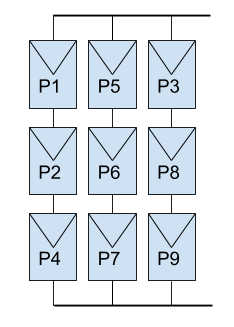
\includegraphics[width=4cm]{MPP3.png} }
\subfloat[]{
	\label{recon-b}
	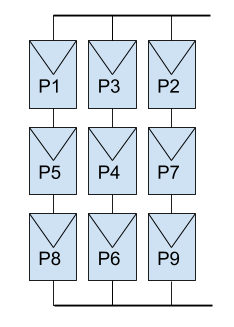
\includegraphics[width=4cm]{MPP4.png}} \\
\caption{Configuration of partial-shading PV array}
\end{figure}

%% \begin{figure}%
%%     \centering
%%     \subfloat[MPP candidate 3]{{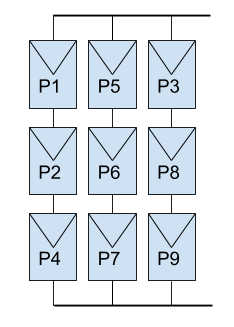
\includegraphics[width=4cm]{MPP3.png} }}%
%% %    \qquad
%%     \subfloat[MPP candidate 4]{{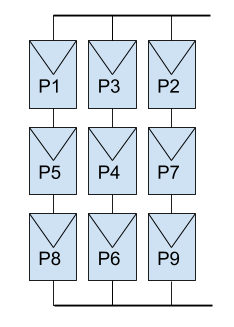
\includegraphics[width=4cm]{MPP4.png} }}%
%%     \caption{Configuration of partial-shading PV array}%
%%     \label{reconfiguration}%
%% \end{figure}


%The general steps of reconfiguration algorithm are presented in Fig. \ref{fig2}. The first step is determine each PV module's \textit{$V_{mpp}$} and \textit{$I_{mpp}$} by using algorithm provided in \cite{b7} \cite{b9}, and calculate MPP current and voltage candidates of PV array. When there are more than two panels connected in series, for a string MPPs is not straightforward. The MPP current and voltage candidates can be evaluated though a procedure presented in \cite{b10}. For string MPP current candidates, \textit{$I_{mpp_n}$} values' different less than 5\% are assumed to be equal. For string MPP voltage candidates, \textit{$V_{mpp_n}$}  can be calculated though multiplay number of active modules (\textit{$N_a$}) by average MPP voltages (\textit{$\bar V_{mpp}$}) with $\pm$18\% error \cite{b10}. Afterward, determine real number of working modules (\textit{$Q_{M_n}$}) for each MPP current candidates by applying method in \cite{b10}. Next, find MPP candidates by multiplying current candidates and voltage candidates which determine by \textit{$Q_{M_n}$}. Due to \textit{$V_{mpp}s$} and \textit{$I_{mpp}s$} can indicate shading distribution among PV array.  Then grouping panels into different shadow distribution.  

%After this procedures is conducted for PV array, all panels will be organized into many groups that from un-shadowed or uniform shadow to fully shadowed group. However, if just simply grouping panels by shadow distribution conditions it may cause electrical connection overhead or unable calculate optimal configuration. To further reconfigure PV system into a better configuration, the replacement part of algorithm will proceed as follow:
%\begin{itemize}
%\item Sorting group by different shadow distribution conditions, select panels from first group into a PV string which working on high current level.
%\item If selected panels' working modules ( \textit{$Q_{M_n}^{*}$} ) less than \textit{$Q_{M_n}$} , select panels from next irradiance level group.
%\item If selected panels' \textit{$Q_{M_n}^{*}$} more than \textit{$Q_{M_n}$}, re-select panels to adjust \textit{$Q_{M_n}^{*}$} equal to \textit{$Q_{M_n}$} if it is possible. 
%\end{itemize}
%\begin{figure}[htbp]
%\centerline{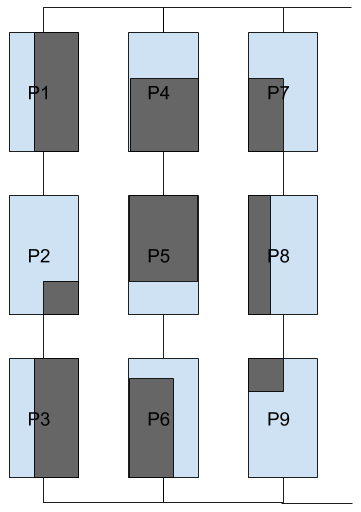
\includegraphics[width=6.2cm]{paper-fig3.png}}
%\caption{An example of un-uniform shadowed PV array.}
%\label{fig3}
%\end{figure}

%This algorithm will better understood by applying to shadow condition showed in Fig. \ref{fig3}. This PV system is composed with 9 PV panels connected into 3 strings as showed in Fig.\ref{fig3}. Irradiance levels, \textit{$I_{mpp}$} and \textit{$V_{mpp}$} of each module are given in Table \ref{tab1}. 

%\begin{table}[]
%\begin{tabular}{cccc}
%\multicolumn{4}{c}{Data of partial-shading PV array} \\
%\\ \hline \hline
%Panels   & Vmpp(V)  & Impp (A)             & MPP(w)  \\ \hline
%P1       &          & {[}0, 0.5, 2{]}      &         \\
%P2       &          & {[}0.5, 3, 3{]}      &         \\
%P3       &          & {[}0.5, 0.5, 0.5{]}  &         \\
%P4       &          & {[}0, 2, 2{]}        &         \\
%P5       &          & {[}0, 0.5, 2{]}      &         \\
%P6       &          & {[}0.5, 2, 2{]}      &         \\
%P7       &          & {[}0.5, 2, 3{]}      &         \\
%P8       &          & {[}2, 2, 2{]}        &         \\
%P9       &          & {[}0.5, 2, 3{]}      &        
%\end{tabular}
%\end{table}
%The example refer to a three-strings PV array, each string contain with 3 panels, each one made of three identical PV modules (\textit{N}=3). In this example, it is assumed that input range of DC-DC converter and MPPT device defined by \textit{$V_{min}$} = 200V and \textit{$V_{max}$} = 500V.  
%\begin{figure}[htbp]
%\centerline{
\includegraphics[width=8cm]{paper-fig4.png}}
%\caption{Organized PV array after first part of Algorithm.}
%\label{fig4}
%\end{figure}
%Due to 5\% error of MPP current candidates and 18\% error of MPP voltage candidates, total error rate of MPP candidates is 23\%. Though procedure of algorithm, MPP candidates with 23\% are: [\{ 0.5, 0.5, 2\}, \{0.5, 2, 2\}, \{2, 2, 2\}, \{2, 2, 3\}] and require working modules per strings are: [\{8, 8, 8\}, \{7, 7, 7\}, \{5, 5, 5\}, \{4, 4, 4\}]. And PV array are organized as Fig.\ref{fig4}
%Those MPP candidates are able to generate maximum output power of PV system, but the configurations of MPP candidates may meet electrical connection overhead. In order to reduce electrical connection simulation time, replacement and feasibility check will be approved. 
%Consider fourth MPP candidate, it require panels on string one working at 2A, panels on string two working at 2A, panels on string three working at 3A and require 4 PV modules working for each string. Firstly, selecting panels for high current string, string three. According to Table \ref{tab1}, only Panel 2, Panel 7 and Panel 9 are able to work at 3A. Those four panel can provide 4 PV module working at 3A and meet requirement of \textit{$Q_{M_n}$}. Because on extra panel can provide module  working on 3A, no replacement will be approved. Means no further improvement for configuration of string three.
%Then select panel for string two, Panel 4 and Panel 8 will be selected, but this configuration is not optimized. Selected panels provide 5 modules able to work at 2A, satisfy requirement of \textit{$Q_{M_n}$} $\ge$ 4, but one module more than requirement. The process will replace Panel 4 by Panel 1 that provide just 4 modules working at 2A. Configuration for string two are Panel 8 and Panel 1. At last, select panels for string one. Panel 4, Panel 5, Panel 6 are selected, they can provide 5 modules working at 2A that satisfy requirement. For configuration on string one due to it is the last string to process and meet requirement, in order to reduce computing time replacement will not be approved. Configuration of MPP candidate \{2, 2, 3\} are \textit{St} 1:\{Panel 4,Panel 5, Panel 6\}, \textit{St} 2: \{Panel 1, Panel 8\}, \textit{St} 3: \{Panel 2, Panel 7, Panel 9\}. As described in section \ref{array}, each string have identical length and Panel 3 not been used in any configuration. So optimized configuration for this MPP candidate are: \textit{St} 1:\{Panel 4,Panel 5, Panel 6\}, \textit{St} 2: \{Panel 1, Panel 8, Panel 3\}, \textit{St} 3: \{Panel 2, Panel 7, Panel 9\}. The MPP values of this configuration calculated by multiplay string voltage and current equal to 347.2W are put into evidence. 

%For the third MPP candidate, as same calculating procedure as fourth MPP candidate, optimized configuration for MPP candidate \{2, 2, 2\} are: \textit{St} 1:\{Panel 4,Panel 8, Panel 3\}, \textit{St} 2: \{Panel 1, Panel 2, Panel 6\}, \textit{St} 3: \{Panel 5, Panel 7, Panel 9\}. 
%
%The first MPP candidate \{0.5, 0.5, 2\}, after replacement string three contain four panels, \{Panel 4, Panel 8, Panel 1, Panel 2\} but it is over maximum string length of this PV array.
%Also for MPP candidate \{0.5, 2, 2\}, there are no configuration can't provide 7 modules working 
%on three different string at 0.5A, 2A, 2A, respectively. 

\section{evaluation of optimization algorithm}
%\subsection{Verification of the Proposed algorithm}
Although the pilot example refers to three strings only, the extension of the method to any number of parallel connected strings is the same.
%This section verifies the effectiveness of proposed algorithm using Matlab simulation. With pilot example presented in last section, shading scenario as showed in Fig.\ref{fig5a}. To minimize power loss, the proposed algorithm, as described, is applied to reconfigure the system. The resulting configuration is depicted in Fig.\ref{fig5b} and Fig.\ref{fig5c}. 
%\begin{figure}%
%    \centering
%    \subfloat[label 1]{{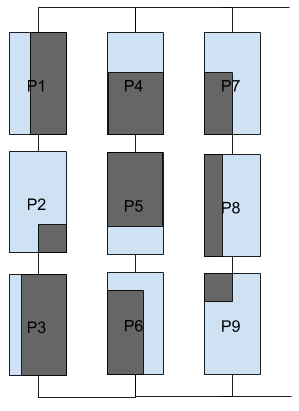
\includegraphics[width=5cm]{paper-fig5(a).png} }}
%    \label{fig5a}
%    \qquad
%    \subfloat[label 2]{{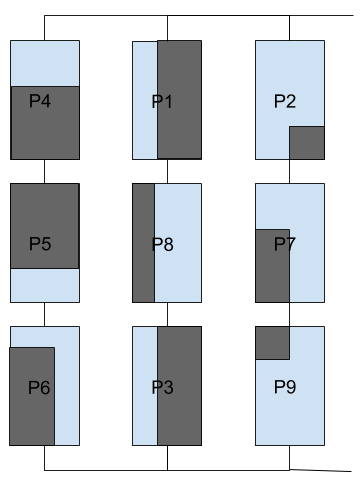
\includegraphics[width=5cm]{paper-fig5(b).png} }}%
%    \qquad
%    \subfloat[label 3]{{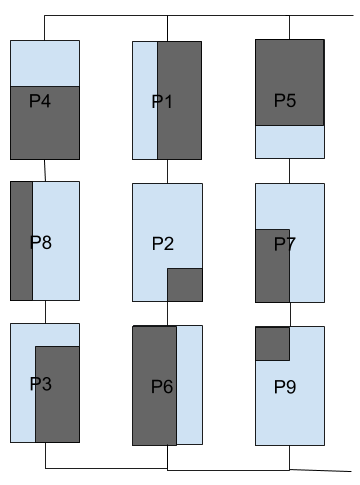
\includegraphics[width=5cm]{paper-fig5(c).png} }}
%    \caption{3 Figures side by side}%
%    \label{fig5c}%
%\end{figure}

%% \begin{figure}
%% \centering 
%% \subfloat[]{
%% 	\label{fig5a}
%% 	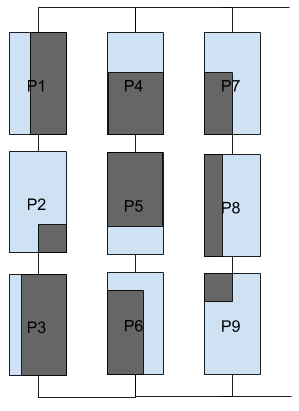
\includegraphics[width=5cm]{paper-fig5(a).png} } \\
%% \subfloat[]{
%% 	\label{fig5b}
%% 	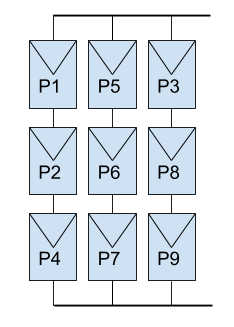
\includegraphics[width=4cm]{MPP3.png} }
%% \subfloat[]{
%% 	\label{fig5c}
%% 	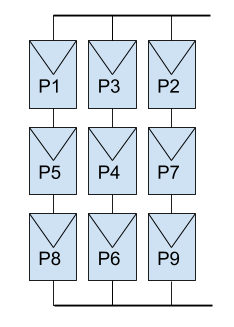
\includegraphics[width=4cm]{MPP4.png}} \\
%% \caption{The PV system under shading scenario (a) before reconfiguration, (b) after reconfiguration for MPP candidate \{2, 2, 2\} and (c) MPP candidate \{2, 2, 3\}} 
%% \end{figure}

%%\begin{figure}[htbp]      
%% \begin{minipage}[t]{0.5\linewidth}
%% \centerline{
\includegraphics{fig2.png}}
%% \caption{(a)}
%% \label{fig5a}
%% %\end{minipage}%
%% %\begin{minipage}[t]{0.5\linewidth}
%% \centerline{
\includegraphics{fig2.png}}
%% \caption{(b)}
%% \label{fig5b}
%% \end{minipage}
%% \end{figure}

As shown in previous section, working modules on each string are large or equal than required \textit{$Q_{M_n}$}, which means mismatched power loss are minimized. The \textit{P-V} curve for this PV array before and after reconfiguration are showed in Fig.\ref{fig6}. It can be seen that after reconfiguration maximum power (283 W and 276W) are higher than before reconfiguration maximum power (277W).

\begin{figure}[htbp]
\centerline{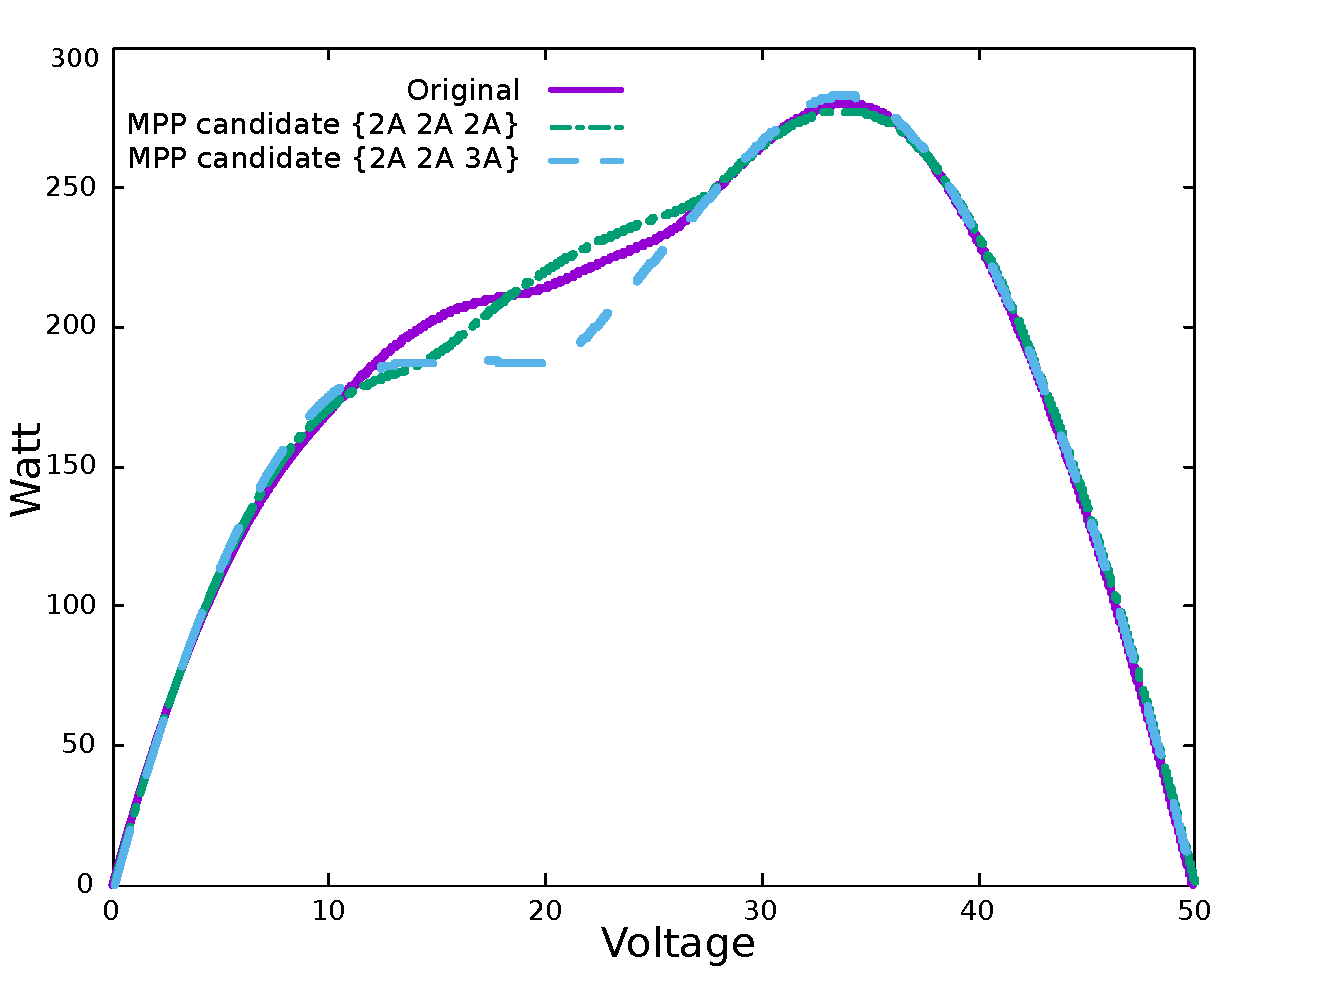
\includegraphics[width=8cm]{zhao.pdf}}
\caption{The \textit{P-V} curves for the PV system under first shading scenario before and after reconfiguration.}
\label{fig6}
\end{figure}

To evaluate the performance of proposed algorithm, we compare the propose algorithm with exhaustive search algorithm for 300 different partial-shading PV arrays. For each PV array, contain 2$\sim$15 PV panels connected into 2$\sim$5 strings. The PV panels will have contain 2$\sim$20 different current candidates. 



The computational time required to find the best configuration and accuracy of configuration in the proposed and exhaustive search algorithm are compared and summarized in Table \ref{tab2}. As shown in Table \ref{tab2}, proposed algorithm achieved high accuracy and less computing time compare with exhaustive search algorithm.
%% and methods described in \cite{b10}. %\cite{b11} \cite{b12}.

\begin{table}[htbp]
\caption{}
\begin{center}
\begin{tabular}{ccc}
\multicolumn{3}{c}{\begin{tabular}[c]{@{}c@{}}COMPARISON BETWEEN EXISTED METHODS\\ AND PROPOSED ALGORITHM\end{tabular}}                                         \\ \hline \hline
\multicolumn{1}{c|}{}                         & \multicolumn{1}{c|}{Proposed Algorithm} & \begin{tabular}[c]{@{}c@{}}Exhaustive search \\ Algorithm\end{tabular} \\ \hline
\multicolumn{1}{c|}{Number of PV Array}       & \multicolumn{2}{c}{300}                                                                                         \\ \hline
\multicolumn{1}{c|}{Number of MPP candidates} & \multicolumn{2}{c}{10961}                                                                                       \\ \hline
\multicolumn{1}{c|}{Feasible Candidates}      & \multicolumn{1}{c|}{1180}              & 1278                                                                   \\ \hline
\multicolumn{1}{c|}{Infeasible Candidates}    & \multicolumn{1}{c|}{9781}              & 9683                                                                   \\ \hline
\multicolumn{1}{c|}{Error Rate}               & \multicolumn{1}{c|}{0.89\%}            & 0\%                                                                    \\ \hline
\multicolumn{1}{c|}{Ave. times per Array}     & \multicolumn{1}{c|}{0.157s}            & 4370s                                                                 
\end{tabular}
\label{tab2}
\end{center}
\end{table}

%The simulations were performed using an Intel i7-4770 3.2-Ghz processor with 32.0 GB of RAM memory. 
The calculation time used by the proposed algorithm for one MPP candidate was 157 ms, which is significantly lower compared with exhaustive search 1hour 12min 50s and accuracy are higher than exhaustive search algorithm.
\section{conclusions}
The existing PV reconfiguration methods either have high accuracy but suffer from long computational time such as exhausted searching algorithm or GA, or they have short computational time but do not guarantee the best configuration as described in \cite{b10}. This paper proposed a new PV system reconfiguration algorithm with feasibility check function and have high accuracy and less computational time. Proposed algorithm's effectiveness has been validated using Matlab simulation. The algorithm was tested though un-uniform shadow distribution among PV array and shows its effectiveness in finding optimal configuration. The proposed algorithm also compared with existed method in terms of accuracy and computational time. The result shows that proposed algorithm has high accuracy and less computational time.
\begin{thebibliography}{00}
\bibitem{b1} Koutroulis, Eftichios, and Frede Blaabjerg. "A new technique for tracking the global maximum power point of PV arrays operating under partial-shading conditions." IEEE Journal of Photovoltaics 2.2 (2012): 184-190.
\bibitem{b2} La Manna, Damiano, et al. "Reconfigurable electrical interconnection strategies for photovoltaic arrays: A review." Renewable and Sustainable Energy Reviews 33 (2014): 412-426.
\bibitem{b3}Storey, Jonathan, Peter R. Wilson, and Darren Bagnall. "The optimized-string dynamic photovoltaic array." IEEE Transactions on Power Electronics 29.4 (2014): 1768-1776.
\bibitem{b4} Storey, Jonathan P., Peter R. Wilson, and Darren Bagnall. "Improved optimization strategy for irradiance equalization in dynamic photovoltaic arrays." IEEE transactions on power electronics 28.6 (2013): 2946-2956.
\bibitem{b5} P. Carotenuto, A. D. Cioppa, A. Marcelli, and G. Spagnuolo, “An evolu- tionary approach to the dynamical reconfiguration of photovoltaic fields,” Neurocomputing, vol. 170, pp. 393–405, 2015.
\bibitem{b6} Carotenuto, Pietro Luigi, et al. "Online recording a PV module fingerprint." IEEE Journal of Photovoltaics 4.2 (2014): 659-668.
\bibitem{b7} Orozco-Gutierrez, M. L., et al. "Fast estimation of MPPs in mismatched PV arrays based on lossless model." Clean Electrical Power (ICCEP), 2015 International Conference on. IEEE, 2015.
%% \bibitem{b8} Spagnuolo, Giovanni, et al. "Control of photovoltaic arrays: Dynamical reconfiguration for fighting mismatched conditions and meeting load requests." IEEE Industrial Electronics Magazine 9.1 (2015): 62-76.
%\bibitem{b9} Carotenuto, Pietro Luigi, et al. "Online recording a PV module fingerprint." IEEE Journal of Photovoltaics 4.2 (2014): 659-668.
\bibitem{b10} Orozco-Gutierrez, M. L., et al. "Optimized configuration of mismatched photovoltaic arrays." IEEE J. Photovolt 6.5 (2016): 1210-1220.
%% \bibitem{b11} El-Dein, MZ Shams, Mehrdad Kazerani, and M. M. A. Salama. "Optimal photovoltaic array reconfiguration to reduce partial shading losses." IEEE Trans. Sustain. Energy 4.1 (2013): 145-153.
%% \bibitem{b12} Storey, Jonathan P., Peter R. Wilson, and Darren Bagnall. "Improved optimization strategy for irradiance equalization in dynamic photovoltaic arrays." IEEE transactions on power electronics 28.6 (2013): 2946-2956.
  
\end{thebibliography}
\end{document}
